% uklad dokumentu
	\documentclass{article}
	\usepackage{xparse}
	\usepackage[margin=1.5cm]{geometry}
    \usepackage{enumerate} 
	\frenchspacing
    \linespread{1.0}
    \setlength{\parindent}{0pt}

% jezyk polski
	\usepackage[T1]{fontenc}
	\usepackage[polish]{babel}
	\usepackage[utf8]{inputenc}
 
% pakiety matematyczne
    \let\lll\undefined
    \usepackage{mathtools}
	\usepackage{amssymb}
    \usepackage{amsthm}
	\usepackage{amsmath}
	\usepackage{amsfonts}
	\usepackage{tikz}
	\usepackage{multirow}

	\usepackage{float}	
	
% pakiety do automatów
	\usetikzlibrary{automata, arrows.meta, positioning, arrows}
	
% wykresiki
	\usepackage{pgfplots}
	\pgfplotsset{compat = newest}
	\usepackage{graphicx}
	\usepackage{subcaption}

    \title{\textbf{Algorytmy Metaheurystyczne\\Komiwojażer Genetycznie}}
    \author{Gabriel Budziński(254609)\\Franciszek Stepek (256310)}
    \date{}
    
    
\begin{document} 
\maketitle

\section*{Przedmowa}
Na samym początku omówimy po krótce naszą implementacje, oraz podamy kilka informacji ogólnych. Następnie bardziej szczegółowo opiszemy poszczególne parametry allgorytmu, a na koniec przedstawimy wyniki i opis wykonywanych eksperymentów. 

\section{Informacje ogólne}
\subsection{Implementacja}
Algorytmy implementujemy w języku \texttt{C/C++}, odległości między wierzchołkami są przechowywane jako pełne tablice dwuwymiarowe typu \texttt{int}, a trasy (pojedyncze osobniki) są w kontenerach \texttt{vector}, co ułatwia operacje odwracania i mieszania.\\
Korzystaliśmy z kompilatora g++ wraz z użyciem flag -lSDL2 (używanej przy wizualizacji, wraz z odpowiednim dla danego systemu operacyjnego podlinkowania do folderu zawierającego) oraz -lpthread (przy korzystaniu z wielowątkowości).\\\\
Dodajmy jeszcze tylko, że jako generatora pseudolosowego użyliśmy typu \texttt{std::mt19937} zdefiniowanego przez \texttt{C++}.

\subsection{Sprzęt}
Programy były testowane na dwóch maszynach, laptopie \textit{Lenovo} i komputerze stacjonarnym. Obie jednostki są wyposażone w procesor architektury \texttt{x86} marki \texttt{intel} oraz 16GB pamięci RAM.
\begin{itemize}
	\item PC - Komputer stacjonarny posiada procesor sześciordzeniowy i5-10600K 4,1 GHz (o obniżonym napięciu operacyjnym).
	\item Laptop - Laptop posiada procesor czterordzeniowy i7-6700HQ 2,6 GHz
\end{itemize}

\subsection{Instancje}
Używaliśmy instancji przygotowanych przez TSPLIB, które dzielą się na 2 kategorie:
\begin{itemize}
	\item 8 instancji symetrycznych:
		\begin{itemize}
			\item berlin52.tsp
			\item st70.tsp
			\item eil76.tsp
			\item bier127.tsp
			\item kroA150.tsp
			\item lin318.tsp
			\item linhp318.tsp
			\item pr439.tsp
		\end{itemize}
	\item 8 instancji asymetrycznych:
		\begin{itemize}
			\item ftv55.atsp
			\item ftv64.atsp
			\item ftv70.atsp
			\item kro124p.atsp
			\item ftv170.atsp
			\item rbg323.atsp
			\item rbg358.atsp
			\item rbg443.atsp
		\end{itemize}
\end{itemize}

W dalszych częściach, instancje będziemy oznaczać przez liczbę mówiącą o rozmiarze problemu (czyli np. st70.tsp oznaczymy jako $n = 70$, albo po prostu $70$) z drobną różnicą - aby rozróżnić lin318 od linhp318, instancję linhp318 będziemy onaczać liczbą $319$.

\subsection{Metodologia/cel}

Testy przeprowadzono za pomocą zaimplementowanych w tym celu funkcji ku jak największej automatyzacji. Dane o przeprowadzonych testach zapisywano do plików tekstowych w formacie CSV, a następnie poddane analizie. Testy i eksperymenty miały na celu zbadanie wydajności naszej implementacji, oraz znalezienie jak najbardziej optymalnych trybów/hiperparametrów dla przypadku ogólnego.

\newpage
\section{Opis parametrów}
W opisie przejdziemy najpierw przez kolejne 'tryby' działania, a następnie omówimy także każdy hiperparametr występujący w naszej implementacji, ale zanim, to wspomnijmy jeszcze tylko, że każda operacja krzyżowania daje nam 2 nowe osobniki.

\subsection{Tryby działania}
\begin{itemize}
	\item StartMode - sposób generowania populacji początkowej:
		\begin{itemize}
			\item 0 - Każdy osobnik jest wybierany z 10 całkowicie losowych (Chodzi o losowe ermutacje dróg)
			\item 1 - Każdy osobnik jest tworzny jako puszczenie algorytmu NearestNeighbor (czyli zachłanne szukanie najbliższego sąsiada z tych co pozostali w każdej iteracji) z losowego punktu startowego
			\item 2 - Hybrydowe połączenie 2 poprzednich, gdzie stosunek losowych do NN wynosi 4:1 (Czyli około 20\% populacji to osobniki 'względnie dobre').
		\end{itemize}

	\item SelectionMode - sposób w jaki jest wykonywana selekcja osobników:
		\begin{itemize}
			\item 0 - Turniejowa, czyli wyieramy najlepszych, a najgorszych odrzucamy
			\item 1 - Kwadratowo ruletkowa - najlepszy osobnik przechodzi dalej, a wszystkim pozostałym przyporządkowywane są wagi względem kwadratu pozycji (Czyli jeżeli mamy populację wielkości 15, to najlepszy przechodzi dalej, kolejny ma wagę $14*14$, później $13*13$ itd., a ostatni ma wagę $1$), a następnie zgodnie z nimi jest robione losowanie.
		\end{itemize}

	\item MutMode - sposób przeprowadzenia mutacji (o jej hiperparametrach będzie później):
		\begin{itemize}
			\item 0 - Mutacja typu \textit{Invert}
			\item 1 - Mutacja typu \textit{Insert}
			\item 2 - Mutacja typu \textit{Swap}
			\item 3 - W każdej iteracji (co to oznacza będzie powiedziane później) losowe wybranie spośród 3 poprzednich
		\end{itemize}

	\item crossMode	- używany operator do krzyżowania osobników:
		\begin{itemize}
			\item 0 - \textit{Order Based Crossover}
			\item 1 - \textit{Modified Order Based Crossover}
			\item 2 - \textit{Partially Mapped Crossover}
		\end{itemize}

	\item crossType - sposób przeprowadzenia i selekcji osobników do krzyżowania:
		\begin{itemize}
			\item 0 - Wszystkie osobniki są ustawione losowo, a następnie krzyżujemy ze sobą 1 z 2, 3 z 4.. itd. Jeżeli osobników było nieparzyście, to ostatni osobnik jest dublowany.
			\item 1 - W każdej iteracji losowana jest para osobników z całej populacji (Ustalona liczba na sztywno, w testach = 20)
			\item 2 - Tak jak poprzednio, ale tym razem liczba losowań jest określona jako rozmiar problemu / 2 (czyli dla $n = 150$ mamy 75 losowań.
		\end{itemize}
\end{itemize}

\subsection{Hiperparametry}
\begin{itemize}
	\item time - czas działania algorytmu - w naszych eksperymentach każde 1 wywołanie trwa 30 sekund
	\item populationSize - rozmiar populacji początkowej (oraz co za tym idzie - rozmiar w każdej iteracji, ponieważ selekcja redukuje rozmiar do rozmiaru początkowego)
	\item mutationThreshold - określa z jakim prawdopodobieństwem zachodzi mutacja (mutacja może zajść podczas tworzenia nowych osobników, rozpatrywana dla każdego z osobna)
	\item mutationIntensification - górne ograniczenie na liczbę pojedynczych mutacji na jednym osobniku (jeżeli zajdzie mutacja, to następnie jest losowana jej intensyfikacja, co najmniej 1, definiuje liczbę iteracji przy mutacji - dlatego przy zastosowaniu MutMode3 może się okazać, że np. wykonają się 3 typu \textit{Invert} oraz 1 typu \textit{Swap})
	\item crossSize - wielkość fragmentu podlegająca krzyżowaniu - przy naszych operatorach jest to wielkość 'wycinka', który definiuje operację krzyżowania
	\item crossCount - wykorzystywane tylko, gdy crossType 1, definiuje liczbę zachodzących krzyżowań
\end{itemize}

\newpage
\section{Opis eksperymentów}
Jako wyniki eksperymentów będziemy pokazywali wartość funkcji celu dla podanych wykonań (Zazwyczaj jako minimum, oraz średnią z 4 wywołań), w formie stosunku wartości względem najlepszej znalezionej (informacja ze strony TSPLIB). Dodatkowo czasami będziemy mówili również o liczbie wykonanych iteracji, aby zastanowić się później nad (ewentualnym) jej wpływem na ostateczny wynik.

\subsection{Poszukiwanie I - Tryb}
Na samym początku przeprowadzony został eksperyment, który miał na celu znalezienie jak najlepszego zestawu trybów dla naszego algorytmu. Użyliśmy tutaj następującego zestawu hiperparametrów (wybranych empirycznie po kilkunastu przetestowaniach algorytmu):
\begin{itemize}
	\item populationSize = 20
	\item mutationThreshold = 0.05
	\item mutationIntensification = 5
	\item crossSize = 7
	\item crossCount = 20
\end{itemize}
Testy wykonaliśmy dla każdej możliwej kombinacji trybów (3*3*2*4*3 = 216), dla każdej z 16 badanych instancji.\\
Przypomnijmy, że czas działania ograniczyliśmy do 30 sekund, a żeby odrobinę zredukować losowy wkład metody, każde wywołanie powtórzyliśmy 4 razy.\\
Pokazanie wszystkich wyników w tabeli byłoby dosyć kłoptliwe i nieczytelne, więc ograniczymy się do kilku mniejszych tabel oraz paru wykresów.\\

\subsubsection{Ogólny rozrzut wyników}
Na początek przedstawimy wykresy pokazujące rozrzut danych dla testów. Na osi Y wartością jest stosunek $\frac{a}{b}$, gdzie:
\begin{itemize}
	\item a - wartość funkcji celu dla pojedynczego eksperymentu
	\item b - najlepsze znalezione rozwiązanie (wg. TSPLIB)
\end{itemize}
Dodatkowo na wykresie zawarta jest też informacja o trybie startującym, dlatego też dla instancji 'a' dane na osi X są na 3 'poziomach': a.0, a.1, a.2, gdzie kolejno oznacza to StartMode.\\

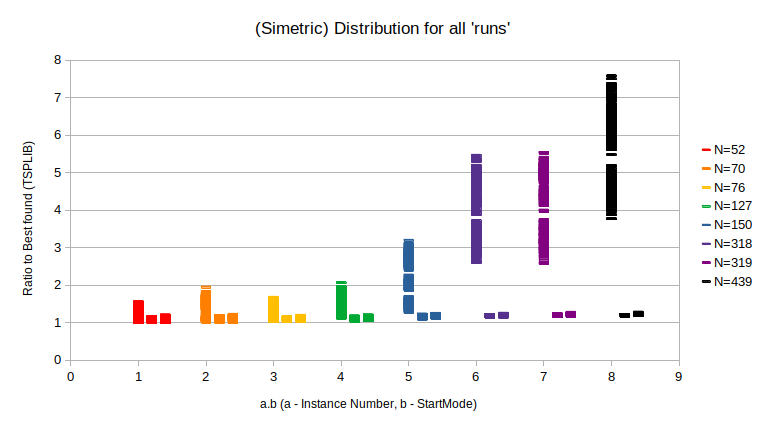
\includegraphics[scale=0.36]{simDistI}
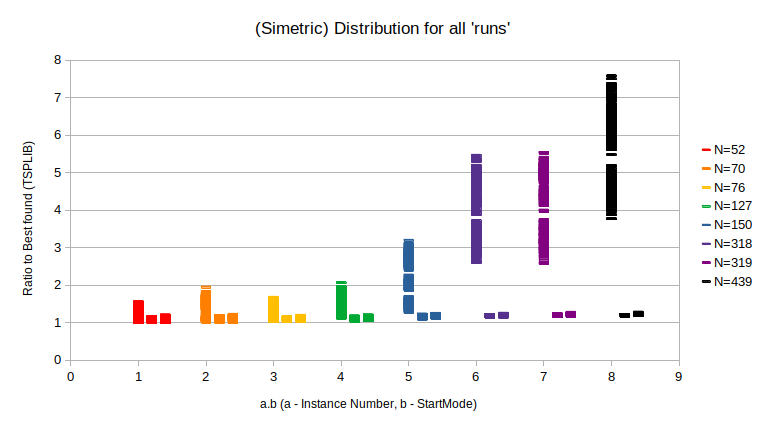
\includegraphics[scale=0.36]{simDistI}

Z podanych wykresów można wyciągnąć dwa zasadnicze wnioski (które aplikują się zarówno do instancji symetrycznych, jak i asymetrycznych):
\begin{itemize}
	\item Jak widać, dla większych instancji algorytm startujący z rozwiązań losowych nie miał wystarczającej ilości czasu, aby dotrzeć do rozwiązań (w sensie wydajności) zbliżonych do pozostałych trybów startowania. Jednak dla instancji mniejszego rozmiaru, z samego tylko wykresu trudno byłoby powiedzieć, czy jego rozwiązania są rzeczywiście gorsze, chociaż  jasno widać, że mają one (losowy start) znacznie większy rozrzut.
	\item Dla większych instancji, pomimo dużego rozrzutu danych, dla samych rozwiązań startujących z całkowicie losowej populacji można wyznaczyć dwie 'grupy', daltego też zaryzykujemy tu swierdzenie, że dla pozostałych trybów startu także to zachodzi (chociaż na razie tego nie widać)
\end{itemize}

\subsubsection{Rozrzut wyników dla poszczególnych instancji}
Jeszcze więcej wykresików!!!\\
Pokażemy teraz dystrybucję wyniku względem liczby iteracji osobno dla każdej instancji. Jednak, nie zawrzemy tutaj wyników, które zostały otrzymane przez użycie całkowicie losowej populacji początkowej, ponieważ tak jak zauważyliśmy na poprzednich wykresach, odbiegają znacznie od pozostałych 2 trybów startujących.

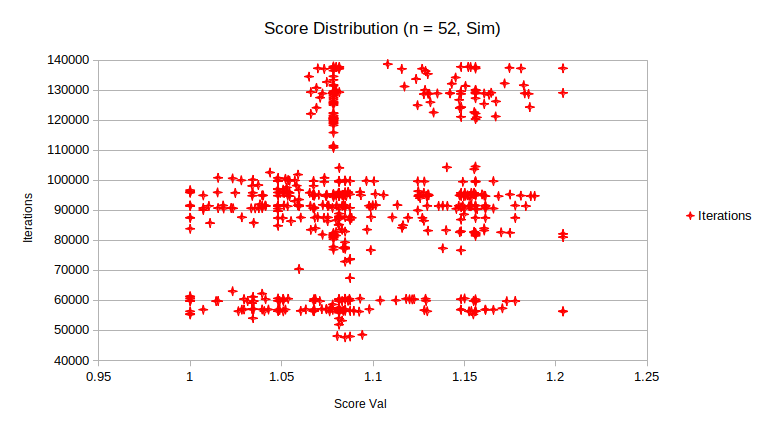
\includegraphics[scale=0.36]{simDist52}
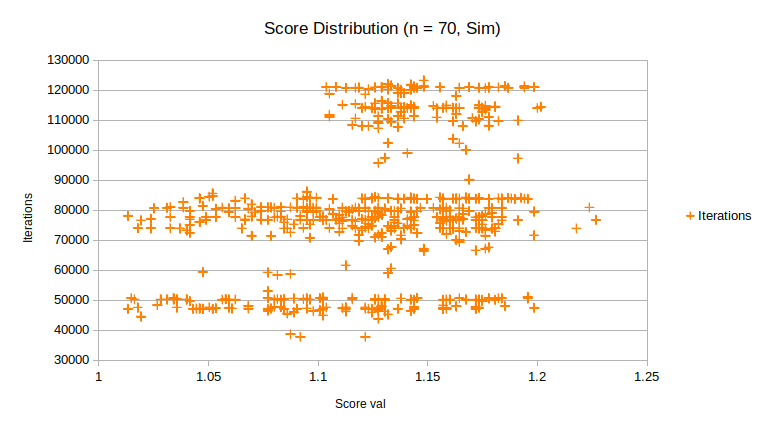
\includegraphics[scale=0.36]{simDist70}
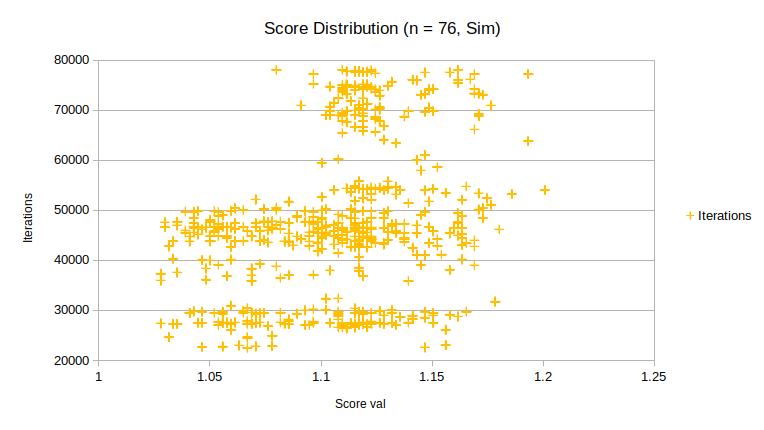
\includegraphics[scale=0.36]{simDist76}
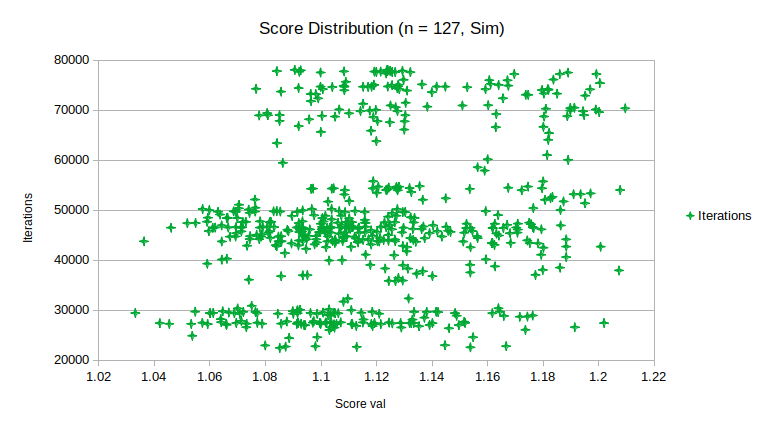
\includegraphics[scale=0.36]{simDist127}
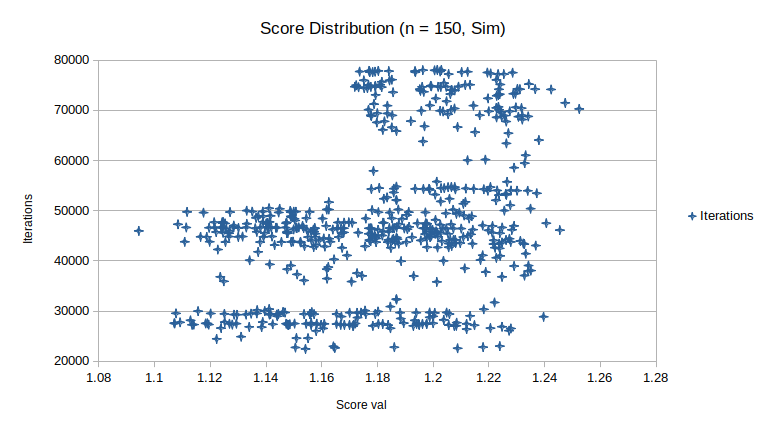
\includegraphics[scale=0.36]{simDist150}
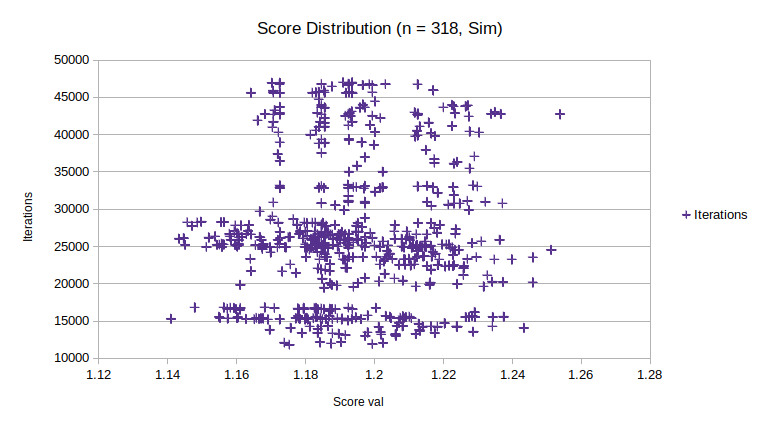
\includegraphics[scale=0.36]{simDist318}
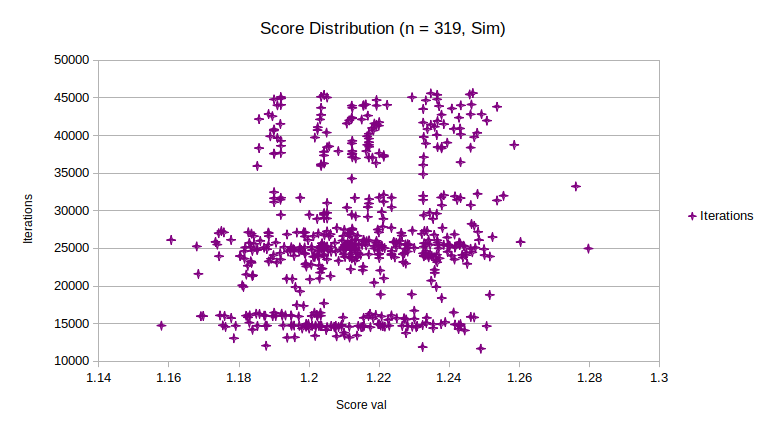
\includegraphics[scale=0.36]{simDist319}
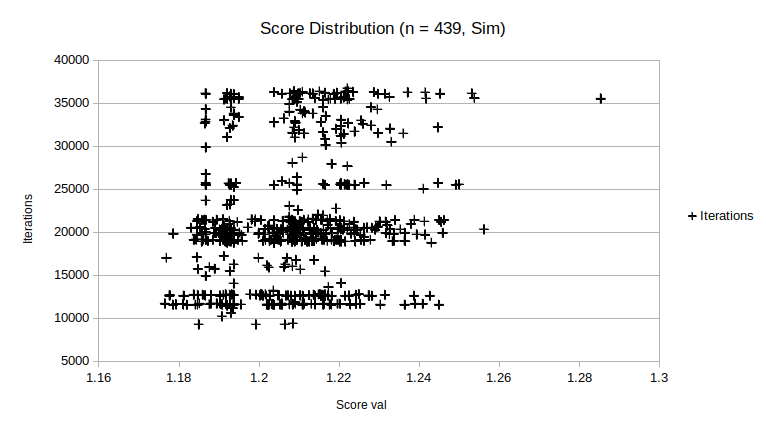
\includegraphics[scale=0.36]{simDist439}
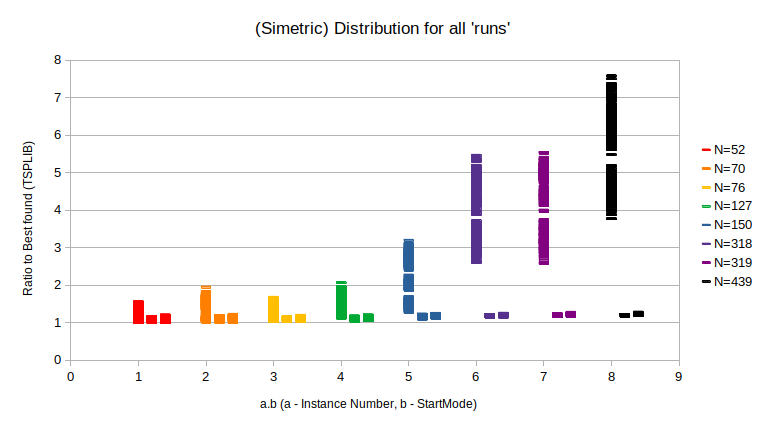
\includegraphics[scale=0.36]{simDistI}
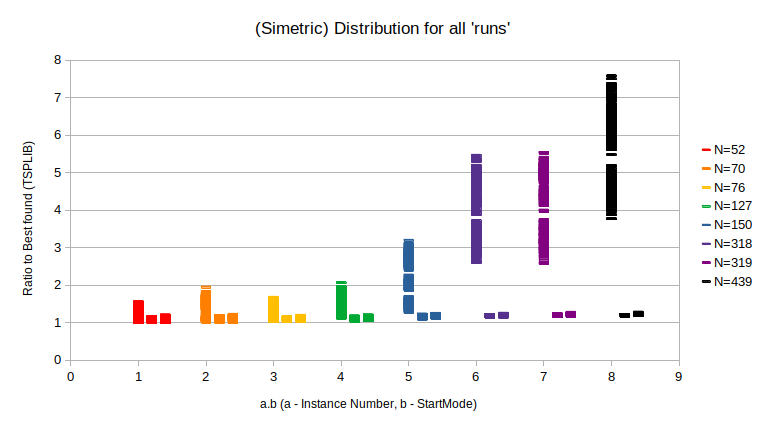
\includegraphics[scale=0.36]{simDistI}
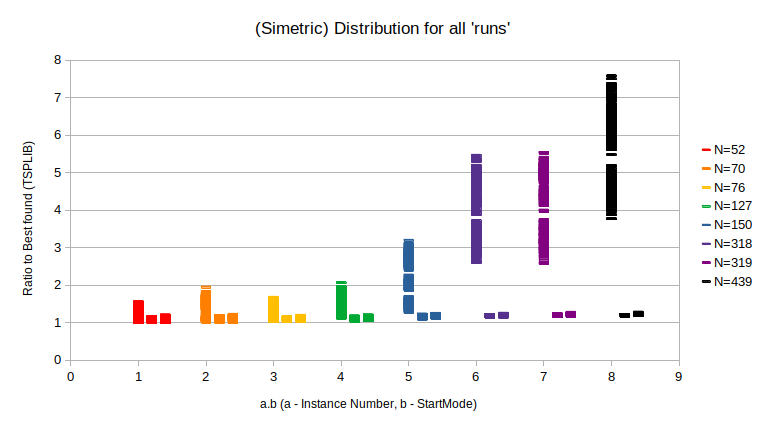
\includegraphics[scale=0.36]{simDistI}
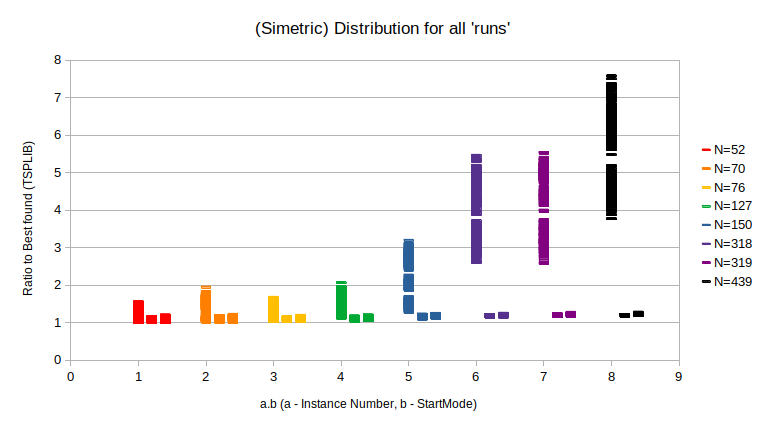
\includegraphics[scale=0.36]{simDistI}
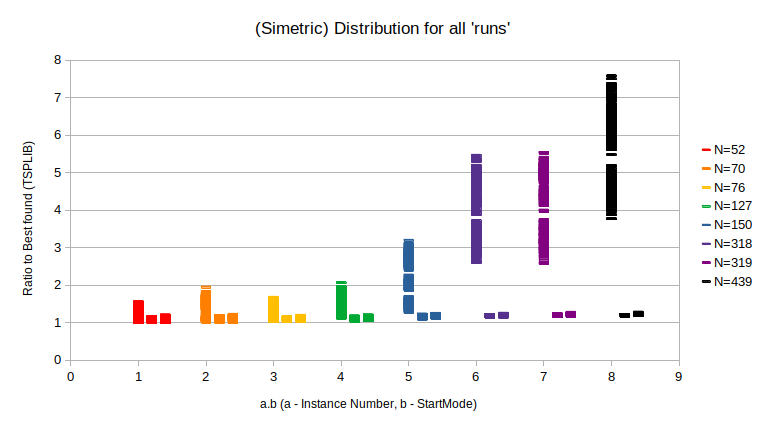
\includegraphics[scale=0.36]{simDistI}
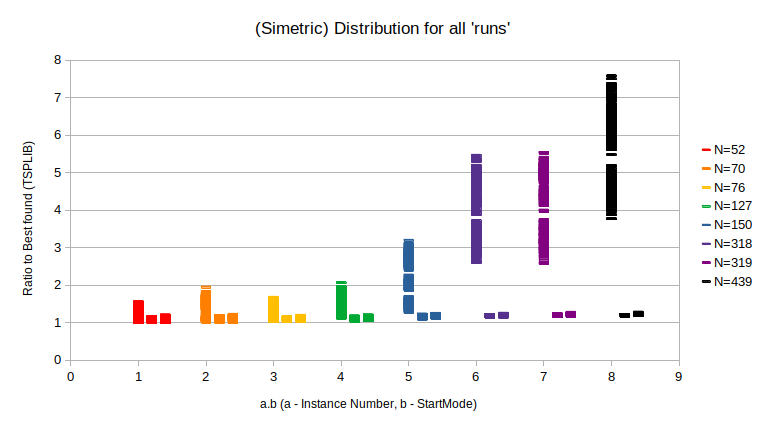
\includegraphics[scale=0.36]{simDistI}
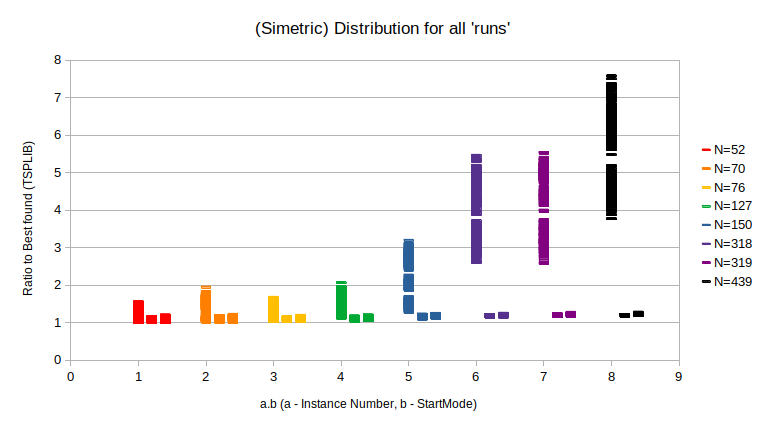
\includegraphics[scale=0.36]{simDistI}
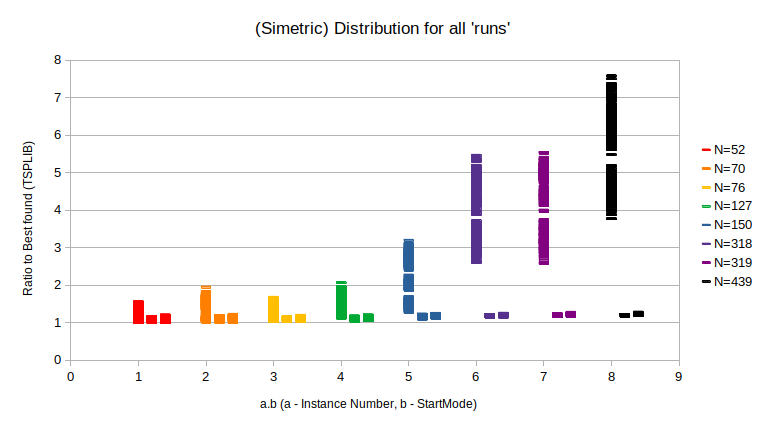
\includegraphics[scale=0.36]{simDistI}

Z tych wykresów wyciągnijmy jeszcze kilka wniosków:
\begin{itemize}
	\item Wniosek 1
	\item Wniosek 2
	\item Wniosek 3
	\item Wniosek 4
	\item Wniosek 5
	\item Wniosek 6
\end{itemize}

\subsubsection{Tryby pod względem jednostkowym}
Pokażemy teraz tabele podsumowującą wszystkie instancje symetryczne, oraz asymetryczne, w której to zawrzemy informacje o minimum i średniej rozwiązań w rozbiciu o każdy tryb (to znaczy, że będziemy patrzeć na całą naszą przestrzeń rozwiązań, a następnie będziemy ją dzielić na rozwiązania względem danego trybu, zatem najpierw (w pierwszych 3 wierszach) podzielimy całość na 3 metody startowe, następnie całość podzielimy na 2 metody selekcji, itd.), z czego wyciągniemy informacje, jakie wartośći danych trybów są ogółem najlepsze gdy się nie bierze pod uwagę kombinacji innych.

\begin{table}[h!]
	\centering
	\begin{tabular}{c|c||c|c||c|c}
Tabela 1. \\
Tryb & Wartość trybu & Min (Sym) & Avg (Sym)  & Min (Asym) & Avg (Asym)\\
\hline
StartMode & 0 & 1 & 2.751 & ? & ?\\
 & 1 & 1 & 1.144 & ? & ?\\
 & 2 & 1 & 1.165 & ? & ?\\
\hline
SelectionMode & 0 & 1 & 1.682 & ? & ?\\
 & 1 & 1 & 1.691 & ? & ?\\
\hline
MutMode & 0 & 1.020 & 1.562 & ? & ?\\
 & 1 & 1 & 1.736 & ? & ?\\
 & 2 & 1.067 & 1.851 & ? & ?\\
 & 3 & 1 & 1.597 & ? & ?\\
\hline
crossMode & 0 & 1.065 & 1.819 & ? & ?\\
 & 1 & 1 & 1.616 & ? & ?\\
 & 2 & 1 & 1.625 & ? & ?\\
\hline
crossType & 0 & 1 & 1.697 & ? & ?\\
 & 1 & 1 & 1.671 & ? & ?\\
 & 2 & 1 & 1.692 & ? & ?\\
	\end{tabular}
\end{table}

Z obu powyższych tabel możemy wyciągnąć następujące wnioski:
\begin{itemize}
	\item Wniosek 1
	\item Wniosek 2
	\item Wniosek 3
\end{itemize}

\subsubsection{10 najlepszych kombinacji}
Teraz spójrzmy jeszcze na ranking 10 najlepszych zestawów parametrów zebranych ze wszystkich instancji.\\
Ranking stworzony został w następujący sposób:
\begin{itemize}
	\item W obrębie każdej instancji:
	\begin{itemize}
		\item Najpierw policzyliśmy minimum oraz średnią z 4 wywołań każdej kombinacji
		\item Później zsumowaliśmy ze sobą obie otrzymane wartości
		\item Następnie posortowaliśmy kombinacje rosnąco względem otrzymanej sumy
		\item Teraz przyporządkowaliśmy miejsca do otrzymanego porządku (przy dublowaniu któregoś z miejsc omijaliśmy kolejne: 32, 32, 34)	
	\end{itemize}
	\item W obrębie typu instancji (symetryczne / asymetryczne),  a później globalnie (wszystkie 16 razem)
	\begin{itemize}
		\item Zsumowaliśmy zajęte miejsca dla każdej kombinacji
		\item posortowaliśmy rosnąco otrzymując ostateczny 'ranking' dla wszystkich kombinacji w obrębie danego typu.	
	\end{itemize}
\end{itemize}

Oto 'główka' dla otrzymanych wyników:
\begin{table}[h!]
	\centering
	\begin{tabular}{c||c|c|c|c|c||c|c}
Tabela 3.\\
Id & StartMode & SelectionMode & MutMode & CrossMode & CrossType & Sum & Avg \\
\hline
107 & 1 & 0 & 3 & 2 & 2 & 98 & 12.25 \\
102 & 1 & 0 & 3 & 1 & 0 & 124 & 15.5 \\
106 & 1 & 0 & 3 & 2 & 1 & 127 & 15.875 \\
103 & 1 & 0 & 3 & 1 & 1 & 141 & 17.625 \\
142 & 1 & 1 & 3 & 2 & 1 & 161 & 20.125 \\
139 & 1 & 1 & 3 & 1 & 1 & 163 & 20.375 \\
140 & 1 & 1 & 3 & 1 & 2 & 188 & 23.5 \\
143 & 1 & 1 & 3 & 2 & 2 & 197 & 24.625 \\
138 & 1 & 1 & 3 & 1 & 0 & 202 & 25.25 \\
104 & 1 & 0 & 3 & 1 & 2 & 206 & 25.75 \\
	\end{tabular}
\end{table}

\begin{table}[h!]
	\centering
	\begin{tabular}{c||c|c|c|c|c||c|c}
Tabela 3. & Pisemnie\\
Id & StartMode & SelectionMode & MutMode & CrossMode & CrossType & Sum & Avg \\
\hline
107 & Hybryda & Turniej & Losowa & Part.Map. & Size/2 & 98 & 12.25 \\
102 & Hybryda & Turniej & Losowa & Mod.Ord.B. & All Par & 124 & 15.5 \\
106 & Hybryda & Turniej & Losowa & Part.Map. & Size/2 & 127 & 15.875 \\
103 & Hybryda & Turniej & Losowa & Mod.Ord.B. & Pop=20 & 141 & 17.625 \\
142 & Hybryda & Ruletka & Losowa & Part.Map. & Pop=20 & 161 & 20.125 \\
139 & Hybryda & Ruletka & Losowa & Mod.Ord.B. & Pop=20 & 163 & 20.375 \\
140 & Hybryda & Ruletka & Losowa & Mod.Ord.B. & Size/2 & 188 & 23.5 \\
143 & Hybryda & Ruletka & Losowa & Part.Map. & Size/2 & 197 & 24.625 \\
138 & Hybryda & Ruletka & Losowa & Mod.Ord.B. & All Par & 202 & 25.25 \\
104 & Hybryda & Turniej & Losowa & Mod.Ord.B. & Size/2 & 206 & 25.75 \\
	\end{tabular}
\end{table}

Z powyższych 3 tabel możemy wyciągnąć następujące wnioski:
\begin{itemize}
	\item Wniosek 1
	\item Wniosek 2
	\item Wniosek 3
\end{itemize}

\subsubsection{Ostatecznie wybrane najlepsze}
Udało się nam teraz wyłonić potencjalnie najlepsze kombinacje trybów (które będziemy stosować później):
\begin{itemize}
	\item Dla wariantu symetrycznego:
	\item Dla wariantu asymetrycznego:
	\item Globalnie:
\end{itemize}

\newpage
\subsection{Poszukiwanie II - hiperparametry}
Po wyznaczeniu rokujących zestawów trybów, przeszliśmy do wyznaczenia jak najlepszych hiperparametrów. W tym celu wyznaczyliśmy 1 zestaw (najlepszy pod względem średniej) dla wariantu symetrycznego, 1 analogicznie dla asymetrycznego, oraz 1 wspólny, który dla obu był w pierwszej 3 (był tylko 1 taki zestaw).\\
Poprzez metodę losowego próbkowania dla każdego hiperparametru (losowy z zakresu podanego zaraz), wykonaliśmy 100 kombinacji, gdzie każdą testowaliśmy 4 razy.\\
Badane instancje:
\begin{itemize}
	\item st70.tsp - sym.
	\item lin318.tsp - sym.
	\item ftv70.atsp - asym.
	\item rbg323.atsp - asym.
\end{itemize}
Badany zakres hiperparametrów:
\begin{itemize}
	\item populationSize : $[10 ; 100]$
	\item mutationThreshold : $[0.0 ; 1.0]$
	\item mutationIntensification : $[1 ; 20]$
	\item crossSize : $[2 ; 20]$
	\item crossCount : $[10 ; 200]$
\end{itemize}
Z przeprowadzonych eksperymentów otrzymaliśmy następujące wyniki:

\subsection{Badanie wpływu zastosowania 'lokalnej poprawy'}
Przy zastosowaniu wyników z 2 poprzednich eksperymentów postanowiliśmy zbadać wpływ działania mechanizmu 'lokalnej poprawy' na wyniki.\\
\textit{Lokalna poprawa} - z pewnym prawdopodobieństwem (określanym parametrem \textit{enhanceChance}) po skończonej mutacji (czyli po szystkich iteracjach) na osobniku wykonujemy algorytm lokalnej poprawy, czyli iteracyjnie przechodzimy przez piątki kolejnych miast i tak modyfikujemy trasę, aby w każdej z tych iteracji przejście było minimalne - zatem najpierw 'poprawiamy' miasta 1-5, potem 2-6 itd. Takich możliwych przejść jest 6 (ponieważ zaczynamy zawsze z 1 i kończymy na 5), zatem jest to w miarę szybkie (dzieje się w czasie liniowym względem liczby miast) i nie powinno znacząco wpływać na liczbę wykonywanych iteracji.\\
W testach wykonaliśmy 10 powtórzeń dla każdej wartości parametru z zakresu $[0.05 ; 1.0]$ ze skokiem o $0.05$. Wyniki przedstawmy na wykresie:

\subsection{Badanie wpływu 'wieku' osobników}
Eksperyment analogiczny do poprzedniego (w sensie metodologii), jednak tym razem badaliśmy wpływ zastosowania wieku na rozwiązanie. Oznaczyliśmy go jako \textit{AgeMax}, przy czym oznacza to, że osobnik będący w populacji dłużej niż \textit{AgeMax} w procesie selekcji jest 'usuwany' z populacji. Zastosowaliśmy tutaj jednak pewną formę elitaryzmu, ponieważ podczas każdej selekcji 'zerujemy' wiek najlepszego osobnika (Najlepszy ma prawo \textit{Picia ze źródła wiecznej młodości}), dzięki czemu go nie tracimy.\\
W testach wykonaliśmy 10 powtórzeń dla każdej wartości z zakresu $[1 ; 20]$, a wyniki przedstawiamy na wykresie:


\subsection{Porównanie najlepszych wyników z algorytmem TabuSearch}
Aby jakoś porównać działanie naszego algorytmu, zestawimy go tutaj z zaimplementoanym algorytmem \textit{TabuSearch}, gdzie Tabu będzie miało następujące parametry:
\begin{itemize}
	\item par1
	\item par2
\end{itemize}
Natomiast \textit{Genetic} otrzymane z eksperymentów z poszukiwaniami. Dla przypomnienia:
\begin{itemize}
	\item par1
	\item par2
\end{itemize}
Testowaliśmy każdą z 16 badanych instancji, oraz każdemu z algorytmów daliśmy budżet czasu równy 90 sekund. Aby jednak dać jakąś szansę (i odrobinę zredukować losowość) algorytmowi genetycznemu, wykonaliśmy dla niego 3 iteracje po 30 sekund. W ten sposób jego wyniki mają szansę być nieco bardziej miarodajne. Wyniki przedstawmy w tabeli:

Oraz jeszcze zobaczmy, co Wilcoxon nam o tym mówi:

\subsection{Badania nad Modelem Wyspowym}

\section{Drobne podsumowanie; Tabele dodatkowe}
Zawrzemy tutaj niepokazane wcześniej tabele z wynikami, oraz pokusimy się o podsumowanie naszych eksperymentów.
\end{document}